\documentclass{article}
\usepackage{amsmath}
\usepackage{amssymb}

\usepackage{tikz}

\usepackage{pgfplots}
\pgfplotsset{compat=1.18}

\usepackage[shortlabels]{enumitem}

\usepackage{graphicx} % Required for inserting images

\title{VL Machine Learning Supervised Techniques}
\author{N/A}
\date{January 2025}

\begin{document}

\maketitle

\section{Exam Questions}

\subsection*{Recurrent Neural Network}
Consider the following recurrent neural network:

\begin{center}
    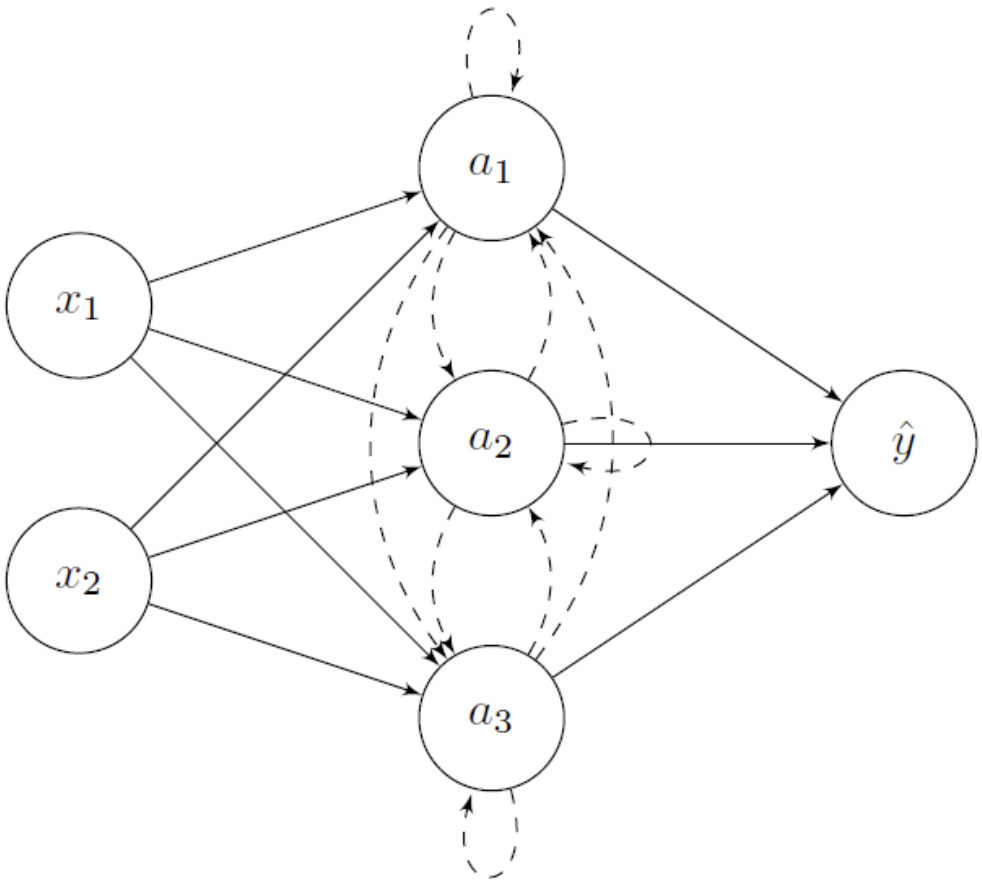
\includegraphics[width=0.7\textwidth]{img/rnn.png}
\end{center}

\[
\text{The activation function in both the hidden layer and in the output layer is ReLU.}
\]

The initial activation vector in the hidden layer is set to:
\[
a(t=0) = \begin{bmatrix} 0 \\ 0 \\ 0 \end{bmatrix}.
\]

The input vector at the first time step is:
\[
x(t=1) = \begin{bmatrix} 1 \\ 2 \end{bmatrix}.
\]
The input vector at the next time step is:
\[
x(t=2) = \begin{bmatrix} 2 \\ 2 \end{bmatrix}.
\]

The input weight matrix is denoted as \( \mathbf{W} \), the recurrent weight matrix as \( \mathbf{R} \), and the output weight matrix as \( \mathbf{V} \). These are given as:

\[
\mathbf{W} = 
\begin{bmatrix}
1 & 0 & 1 \\
1 & 1 & 1
\end{bmatrix}, \quad
\mathbf{R} = 
\begin{bmatrix}
0 & 1 & 1 \\
1 & 0 & 1 \\
1 & 1 & 0
\end{bmatrix}, \quad
\mathbf{V} = 
\begin{bmatrix}
1 & -1 & 1
\end{bmatrix}.
\]

Compute the forward pass and calculate the network outputs \( \hat{y}(t=1) \) and \( \hat{y}(t=2) \).

\subsection*{Convolution}
Consider the input image:

\[
\mathbf{x} =
\begin{bmatrix}
0 & 1 & 2 & 1 & 2 \\
1 & 2 & -1 & 0 & 0 \\
0 & 0 & 0 & 0 & 1 \\
2 & 1 & -1 & 0 & 2 \\
2 & 0 & 2 & 0 & -1 \\
0 & 2 & 2 & -1 & 2 \\
0 & 2 & 1 & -1 & 0
\end{bmatrix}
\]

and the filter:

\[
\mathbf{W} =
\begin{bmatrix}
0 & 1 & 0 \\
0 & 0 & 1 \\
1 & 0 & 0
\end{bmatrix}.
\]

Let \(\mathbf{s} = \mathbf{W} \ast \mathbf{x}\).

Notation: Let \(s_{i,j}\) denote the entry of \(\mathbf{s}\) in row \(i\) and column \(j\). Indices start at 1 (i.e., \(s_{1,1}\) denotes the top-left entry of \(\mathbf{s}\)).

The values inserted for the padding operation shall all be zeros!

\begin{itemize}
    \item Assuming stride equal to 2 and padding equal to 1, compute \(s_{3,3}\).
    \item Assuming stride equal to 2 and padding equal to 1, the output matrix has \(d_r\) rows and \(d_c\) columns. Compute \(d_r\).
    \item Assuming stride equal to 1 and padding equal to 0, the output matrix has \(D_r\) rows and \(D_c\) columns. Compute \(D_c\).
\end{itemize}

\subsection*{Perceptron}

Which statements are true? Multiple answers are possible!

\begin{enumerate}[(a)]
    \item The perceptron learning algorithm tries to find the optimal weights for a linear threshold unit.
    \item Dropout is a regularization technique where random data features are set to zero during training.
    \item Backpropagation is a recursive procedure so that knowing gradients of weights in lower layers allows for computing the gradients in upper layers.
    \item For weight decay, a regularization term that measures the overall weight size is added to the objective.
    \item The vanishing gradient problem for feed-forward networks can be tackled by choosing appropriate weight initializations.
\end{enumerate}

\subsection*{Boosting}
Consider the following datapoints \(\mathbf{x}\) and labels \(\mathbf{y}\):
\[
\mathbf{x} = \begin{bmatrix} 0 & 1 & 2 & 3 & 4 \end{bmatrix}, \quad
\mathbf{y} = \begin{bmatrix} 0 & 0 & 1 & 1 & 0 \end{bmatrix}.
\]

You want to do boosting and therefore aggregate several weak classifiers. Following the AdaBoost algorithm, you modify the weights of the data points and the weights of the models in the ensemble in each iteration step.

Assume that the first model classifies all data greater than 1.5 with 1 and 0 otherwise. Mark the changes of the weights of the individual data points:

\begin{itemize}
    \item Point \(x = 0\): 
    \item Point \(x = 1\): 
    \item Point \(x = 2\): 
    \item Point \(x = 3\): 
    \item Point \(x = 4\): 
\end{itemize}

In the second iteration step, we use a model that classifies datapoints greater than 2.5 with 0 and 1 otherwise. Mark the changes of the weights of the individual data points:

\begin{itemize}
    \item Point \(x = 0\): 
    \item Point \(x = 1\): 
    \item Point \(x = 2\): 
    \item Point \(x = 3\): 
    \item Point \(x = 4\): 
\end{itemize}

In the final aggregation, which model is assigned the larger weight?

\subsection*{Neural Networks}

\begin{center}
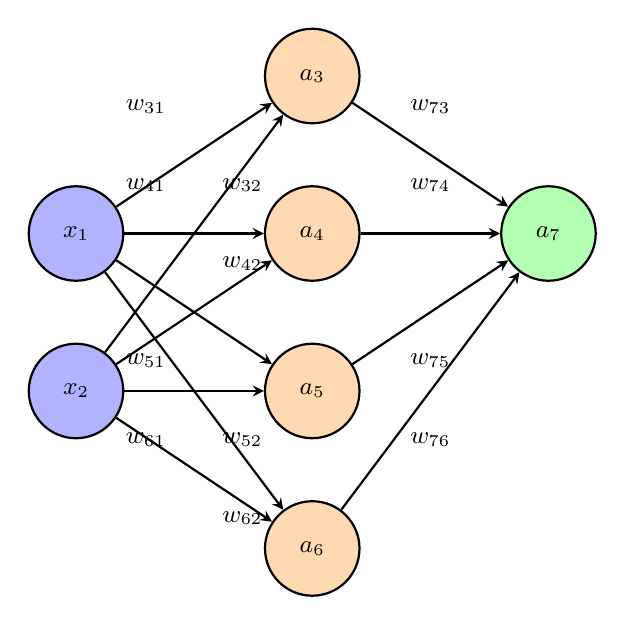
\begin{tikzpicture}[
    every node/.style={circle, draw, minimum size=1.2cm, font=\small},
    weight/.style={font=\small, draw=none, rectangle},
    ->, >=stealth, thick
]

% Input layer
\node[fill=blue!30] (x1) at (0, 4) {$x_1$};
\node[fill=blue!30] (x2) at (0, 2) {$x_2$};

% Hidden layer
\node[fill=orange!30] (a3) at (3, 6) {$a_3$};
\node[fill=orange!30] (a4) at (3, 4) {$a_4$};
\node[fill=orange!30] (a5) at (3, 2) {$a_5$};
\node[fill=orange!30] (a6) at (3, 0) {$a_6$};

% Output layer
\node[fill=green!30] (a7) at (6, 4) {$a_7$};

% Connections from input layer to hidden layer
\draw (x1) -- (a3) node[midway, above left, weight] {$w_{31}$};
\draw (x1) -- (a4) node[midway, above left, weight] {$w_{41}$};
\draw (x1) -- (a5) node[midway, below left, weight] {$w_{51}$};
\draw (x1) -- (a6) node[midway, below left, weight] {$w_{61}$};

\draw (x2) -- (a3) node[midway, above right, weight] {$w_{32}$};
\draw (x2) -- (a4) node[midway, above right, weight] {$w_{42}$};
\draw (x2) -- (a5) node[midway, below right, weight] {$w_{52}$};
\draw (x2) -- (a6) node[midway, below right, weight] {$w_{62}$};

% Connections from hidden layer to output layer
\draw (a3) -- (a7) node[midway, above, weight] {$w_{73}$};
\draw (a4) -- (a7) node[midway, above, weight] {$w_{74}$};
\draw (a5) -- (a7) node[midway, below, weight] {$w_{75}$};
\draw (a6) -- (a7) node[midway, below, weight] {$w_{76}$};

\end{tikzpicture}
\end{center}

The input unit 1 has activation \(\mathbf{x}\). The preactivations of the hidden units \(i = 3, 4, 5, 6\) are denoted as \(s_i\) and their activations as \(a_i\), respectively.

The preactivation of the output unit 7 is denoted as \(s_7\) and the output as \(\hat{y} = a_7\). The true label is denoted as \(y\). There are no biases.

In the hidden layer, we use ReLU as the activation function, i.e.,
\[
f(s) = \text{ReLU}(s) = \max(0, s).
\]
In the output layer, the activation is the identity function.

The delta-errors at the output are denoted as \(\delta_7\), and the hidden delta-errors as \(\delta_3, \delta_4, \delta_5, \delta_6\), respectively.

As a loss function, we use the squared error:
\[
L(y, \hat{y}) = \frac{1}{2}(y - \hat{y})^2.
\]

The learning rate is denoted as \(\eta\). The network weights are updated via backpropagation and gradient descent, and these updated weights are denoted by a superscript ``new".

We are given the input value, the current network weights, the true label, and the learning rate for gradient descent update:

\[
\begin{aligned}
    x_1 &= 2.0, \quad x_2 = 3.0, \\
    w_{31} &= 1.0, \quad w_{41} = -1.0, \quad w_{51} = 3.0, \quad w_{61} = -3.0, \\
    w_{32} &= 2.0, \quad w_{42} = -2.0, \quad w_{52} = 4.0, \quad w_{62} = -4.0, \\
    w_{73} &= 1.0, \quad w_{74} = 2.0, \quad w_{75} = -3.0, \quad w_{76} = 4.0, \\
    y &= -11.0, \quad \eta = 0.05.
\end{aligned}
\]

\textbf{Task:} Compute the following quantities (forward pass and backpropagation). The result are integers:
\begin{itemize}
    \item \(\hat{y}\)
    \item \(\frac{\partial L}{\partial w_{73}}\)
    \item \(w^{\text{new}}_{73}\)
    \item \(\frac{\partial L}{\partial w_{51}}\)
\end{itemize}

\subsection*{Logistic Regression}

Which statements are true? Multiple answers are possible!

\begin{enumerate}[(a)]
    \item The parameters in logistic regression are always positive.
    \item The maximum-likelihood approach assumes that the data samples all originate from the same distribution.
    \item Logistic regression also works for multi-dimensional and non-binary inputs.
    \item Any number between -1 and 1 can be an output of the sigmoid function.
    \item Stochastic gradient descent provides a cheaper estimate of a gradient by using only a fraction of the training samples.
    \item Logistic regression can only be used for normally (Gauss) distributed input data.
    \item The gradients $\frac{\partial L}{\partial W}$ of the logistic regression objective cannot be computed analytically.
\end{enumerate}

\subsection*{Generalization, Underfitting, and Overfitting}

Which of the following statements are correct?

Select one or more:

\begin{enumerate}[(a)]
    \item The generalization error is also called empirical risk.
    \item The training data set and the test data set should be i.i.d., i.e., they should be distributed as if they were drawn independently from the same distribution.
    \item The training data set and the test data set have to be disjoint, i.e., they must have no data samples in common.
    \item Any two data sets that are independent are useful as test and training data sets.
    \item Underfitting is indicated if the model performs better on the test data set than on the training data set.
    \item If a model is overfitting, its performance on the test data set is typically worse than on the training data set.
\end{enumerate}

\subsection*{Bias-Variance Tradeoff in Polynomial Regression}

\begin{center}
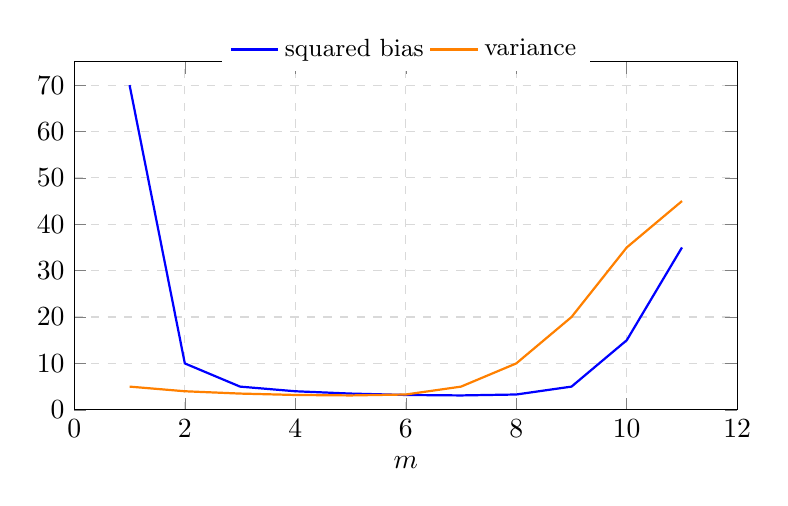
\begin{tikzpicture}
    \begin{axis}[
        width=10cm,
        height=6cm,
        xlabel={$m$},
        ylabel={},
        xmin=0, xmax=12,
        ymin=0, ymax=75,
        xtick={0, 2, 4, 6, 8, 10, 12},
        ytick={0, 10, 20, 30, 40, 50, 60, 70},
        grid=major,
        grid style={dashed,gray!30},
        legend style={font=\small, draw=none, at={(0.5,1.1)}, anchor=north, legend columns=-1},
        legend entries={squared bias, variance}
    ]
        % Squared Bias Data
        \addplot[color=blue, thick] coordinates {
            (1, 70) (2, 10) (3, 5) (4, 4) (5, 3.5) (6, 3.2) (7, 3.1) (8, 3.3) (9, 5) (10, 15) (11, 35)
        };
        % Variance Data
        \addplot[color=orange, thick] coordinates {
            (1, 5) (2, 4) (3, 3.5) (4, 3.2) (5, 3.1) (6, 3.3) (7, 5) (8, 10) (9, 20) (10, 35) (11, 45)
        };
    \end{axis}
\end{tikzpicture}
\end{center}
Assume that we applied polynomial regression with degree \(m = 1, \ldots, 11\) to a noisy data set. The above diagram visualizes the squared bias and the model variance for different values of \(m\). Tick the correct statements.

Select one or more:

\begin{enumerate}[(a)]
    \item For values \(m \leq 3\), the model seems to be too simple to fit the training data. This is an instance of overfitting.
    \item Too small model class complexity leads to underfitting.
    \item Too large model class complexity leads to overfitting as can be seen by the small (squared) bias.
    \item In general, the higher the polynomial degree, the better the model performance.
    \item Models with degree \(m \geq 7\) seem to have good generalization properties due to their low bias.
    \item For appropriate model class complexity, i.e., \(3 \leq m < 7\), both model variance and bias are low, which indicates good generalization abilities.
\end{enumerate}

\subsection*{Constrained Optimization Problem}

Find the solution \(\hat{w}_1, \hat{w}_2\) to the following constrained optimization problem with respect to \(w_1, w_2\):

\[
\text{minimize} \quad \frac{1}{2}(w_1^2 + w_2^2)
\]
\[
\text{subject to} \quad 2 - w_1 - 2w_2 \leq 0.
\]

You can use a pocket calculator. Give the answer as a real number, rounded to one decimal place. Use ``.'' or ``,'' for the decimal point (depending on what works with your system). Number format example: \(1.2\) or \(1,2\).

\begin{itemize}
    \item \(\hat{w}_1 =\)
    \item \(\hat{w}_2 =\)
\end{itemize}

\subsection*{Gini Impurity Gain in Decision Trees}

\begin{center}
\begin{tikzpicture}
    \begin{axis}[
        width=10cm,
        height=7cm,
        xlabel={$x_1$},
        ylabel={$x_2$},
        xmin=0, xmax=10,
        ymin=0, ymax=7,
        grid=major,
        grid style={dashed,gray!30},
        legend pos=north east,
        legend style={draw=none, font=\small},
        scatter/classes={
            orange={mark=o,draw=orange,fill=orange},
            blue={mark=*,draw=blue,fill=blue}
        }
    ]
        % Data points
        \addplot[scatter,only marks,scatter src=explicit symbolic]
        table[meta=label] {
            x y label
            5 4 orange
            7 3 blue
            6 6 orange
            1 2 orange
            9 5 blue
            4 1 blue
        };
        \legend{+1 (orange), -1 (blue)}
    \end{axis}
\end{tikzpicture}
\end{center}

The figure above displays labeled points in two dimensions, where the orange points are labeled with \(+1\) and the blue ones with \(-1\), respectively. Assume that you want to fit a decision tree to it, where you make the first split at \(x_1 = 6.5\). Compute the Gini impurity gain of this split.

You can use a pocket calculator. Give the answer as a real number, rounded to two decimal places. Use ``.'' or ``,'' for the decimal point. Number format example: \(1.23\).

\textbf{Answer:} 

\subsection*{AdaBoost: Weight Update Problem}

\begin{center}
\begin{tikzpicture}
    \begin{axis}[
        width=10cm,
        height=7cm,
        xlabel={$x_1$},
        ylabel={$x_2$},
        xmin=0, xmax=10,
        ymin=0, ymax=7,
        grid=major,
        grid style={dashed,gray!30},
        legend pos=north east,
        legend style={draw=none, font=\small},
        scatter/classes={
            orange={mark=o,draw=orange,fill=orange},
            blue={mark=*,draw=blue,fill=blue}
        }
    ]
        % Data points
        \addplot[scatter,only marks,scatter src=explicit symbolic]
        table[meta=label] {
            x y label
            5 4 orange
            7 3 blue
            6 6 orange
            1 2 orange
            9 5 blue
            4 1 blue
        };
        \legend{+1 (orange), -1 (blue)}
    \end{axis}
\end{tikzpicture}
\end{center}

The figure above shows labeled points in two dimensions, where the orange points are labeled with \(+1\) and the blue ones with \(-1\), respectively. We want to classify the datapoints using the AdaBoost algorithm, where we assume all the points to have uniform weights at the beginning. Assume that the first model we choose is given by:

\[
g_1(\mathbf{x}) = 
\begin{cases} 
+1 & \text{if } x_2 > 3.5 \\ 
-1 & \text{else.}
\end{cases}
\]

What are the \((x_1, x_2)\)-coordinates of the points whose weight will increase as a result of incorporating \(g_1\) (i.e., of the weight update due to \(g_1\))?

\textbf{Select one or more:}

\begin{itemize}
    \item \((5, 4)\)
    \item \((7, 3)\)
    \item \((6, 6)\)
    \item \((1, 2)\)
    \item \((9, 5)\)
    \item \((4, 1)\)
\end{itemize}

\subsection*{Random Forests}

Which of the following statements about Random Forests are correct?

\textbf{Select one or more:}

\begin{enumerate}[(a)]
    \item A new bootstrap subsample of the training data set is drawn at each individual split during training of a tree.
    \item A new subsample of considered features from the training data set is drawn at each individual split during the training of a tree.
    \item For out of bag estimates for each observation \(z_i\), one constructs the RF predictor by averaging only trees corresponding to bootstrap samples in which the observations \(z_i\) did appear.
    \item A simple strategy to equalize the importance of classes and, thereby, to improve balanced accuracy instead of standard accuracy is to stratify classes when sampling.
    \item The subsample of considered features from the training data set is drawn at the beginning of the training of a new tree and kept constant throughout the training procedure of this tree.
    \item The subsample of considered features from the training data set is drawn at the beginning of the training of a Random Forest and kept constant throughout the training procedure of the whole Random Forest.
\end{enumerate}

\subsection*{Logistic Regression}

Which of the following statements about Logistic Regression are correct?

\textbf{Select one or more:}

\begin{enumerate}[(a)]
    \item The optimal weights of a Logistic Regression model cannot be directly calculated; instead, optimization algorithms are typically used for this purpose.
    \item Due to the non-linearity of the sigmoid function, a Logistic Regression model is able to perfectly solve the XOR problem.
    \item Logistic regression models the linear relationship between a categorical label and some features.
    \item When training a Logistic Regression classifier, one might get stuck in a local minimum of the loss, which may yield sub-optimal performance.
    \item The loss function used in Logistic Regression is the cross-entropy loss. Every minimum of this loss function is a global minimum due to it being convex.
\end{enumerate}

\subsection*{Neural Network: Backpropagation and Delta-Errors}

The following neural network has the specified weights:

For the first layer (\( W^{(1)} \)):

\[
W^{(1)} =
\begin{bmatrix}
w_{41} & w_{42} & w_{43} \\
w_{51} & w_{52} & w_{53}
\end{bmatrix}
=
\begin{bmatrix}
-3 & 0 & -1 \\
0.5 & 0.5 & -0.5
\end{bmatrix}
\]

For the second layer (\( W^{(2)} \)):

\[
W^{(2)} =
\begin{bmatrix}
w_{64} & w_{65}
\end{bmatrix}
=
\begin{bmatrix}
5 & 0.5
\end{bmatrix}
\]



\begin{center}
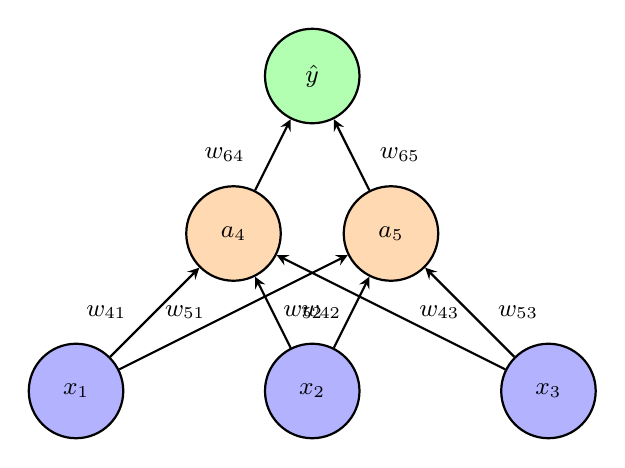
\begin{tikzpicture}[
    every node/.style={circle, draw, minimum size=1.2cm, font=\small},
    weight/.style={font=\small, draw=none, rectangle},
    ->, >=stealth, thick
]

% Input layer
\node[fill=blue!30] (x1) at (0, 0) {$x_1$};
\node[fill=blue!30] (x2) at (3, 0) {$x_2$};
\node[fill=blue!30] (x3) at (6, 0) {$x_3$};

% Hidden layer
\node[fill=orange!30] (a4) at (2, 2) {$a_4$};
\node[fill=orange!30] (a5) at (4, 2) {$a_5$};

% Output layer
\node[fill=green!30] (y) at (3, 4) {$\hat{y}$};

% Connections from input to hidden layer
\draw (x1) -- (a4) node[midway, left, weight] {$w_{41}$};
\draw (x1) -- (a5) node[midway, left, weight] {$w_{51}$};

\draw (x2) -- (a4) node[midway, right, weight] {$w_{42}$};
\draw (x2) -- (a5) node[midway, left, weight] {$w_{52}$};

\draw (x3) -- (a4) node[midway, right, weight] {$w_{43}$};
\draw (x3) -- (a5) node[midway, right, weight] {$w_{53}$};

% Connections from hidden to output layer
\draw (a4) -- (y) node[midway, left, weight] {$w_{64}$};
\draw (a5) -- (y) node[midway, right, weight] {$w_{65}$};

\end{tikzpicture}
\end{center}


The preactivations of the hidden units are denoted as \(s_4\) and \(s_5\) from left to right, and their activations as \(a_4\) and \(a_5\), respectively. In the hidden layer, we use ReLU as the activation function, i.e., \(f_4(x) = f_5(x) = \text{ReLU}(x) = \max(0, x)\). In the output layer, the activation is the identity function. The preactivation of the output layer is denoted as \(s_6\) and the output as \(a_6 = \hat{y}\). The delta-error at the output is denoted as \(\delta_6\), and the hidden delta-errors as \(\delta_4\) and \(\delta_5\) from left to right, respectively. The true label is \(y = 1\), and as the loss function, we use the mean-squared loss, i.e., 

\[
L(y, \hat{y}) = \frac{1}{2}(y - \hat{y})^2.
\]

Compute the following quantities:

\begin{itemize}
    \item \(a_6 = \hat{y}:\)
    \item \(\delta_4:\)
    \item \(\delta_5:\)
    \item \(\frac{\partial L}{\partial s_5}:\)
\end{itemize}

You can use a pocket calculator. Give the answer as a real number, rounded to two decimal places. Use ``.'' or ``,'' for the decimal point (depending on what works with your system). Number format example: 1.23 or 1,23.

\subsection*{Generalization Error and Empirical Risk}

Which statements about the generalization error and the empirical risk are true?

\textbf{Multiple answers are possible!}

\begin{itemize}
    \item[(a)] The generalization error is the expected loss on future data for a given model.
    \item[(b)] The generalization error has the form 
    \[
    \int_X \int_{\mathbb{R}} L(y, g(\vec{x}; \vec{w})) p(\vec{x}) p(y) \, dy \, d\vec{x}.
    \]
    \item[(c)] The empirical risk on a dataset with $n$ samples has the form 
    \[
    R_{\text{emp}} = \frac{1}{n} \prod_{i=1}^n L(y_i, g(\vec{x}_i; \vec{w})).
    \]
    \item[(d)] A common assumption for estimation of the generalization error via the empirical risk is that data are independent and identically distributed (i.i.d.).
    \item[(e)] A good estimation of the generalization error via the empirical risk generally requires that data points are uniformly distributed.
    \item[(f)] A good estimation of the generalization error via the empirical risk generally requires a large number of samples.
    \item[(g)] A good estimation of the generalization error via the empirical risk generally requires use of a differentiable loss function.
    \item[(h)] Estimating the risk via samples from a test set, which have not been used in training, avoids the problem of underfitting.
\end{itemize}

\subsection*{Supervised Machine Learning}

Which statements about supervised machine learning are true?

\textbf{Multiple answers are possible!}

\begin{itemize}
    \item[(a)] Having a small training error but a large test error indicates overfitting.
    \item[(b)] Bias increases with increasing model class complexity.
    \item[(c)] ROC curves allow to evaluate a classifier independent of class distribution and independent of misclassification cost.
    \item[(d)] Model variance decreases with increasing model class complexity.
    \item[(e)] Supervised machine learning uses data with supervisory signals (i.e. labels) for predictive modeling.
    \item[(f)] The more degrees of freedom, the lower the risk to fit to noise.
    \item[(g)] The Bayes Optimal Classifier is a probabilistic model that makes the most probable prediction for a new sample.
    \item[(h)] Supervised machine learning uses explicit knowledge to design models deductively.
\end{itemize}

\subsection*{Probabilistic Framework and Bayes Optimal Classifier}

Which statements about the probabilistic framework and the Bayes optimal classifier are true?

\textbf{Multiple answers are possible!}

\begin{itemize}
    \item[(a)] Using the zero-one loss and binary classification, the minimal risk is given by 
    \[
    \int_X \min\big(p(y = -1 \mid \mathbf{x}), p(y = +1 \mid \mathbf{x})\big) p(\mathbf{x}) \, d\mathbf{x}.
    \]
    \item[(b)] Bayes Theorem reads: 
    \[
    p(b \mid a) = \frac{p(a \mid b) p(a)}{p(b)}.
    \]
    \item[(c)] The Bayes Optimal Classifier minimizes the misclassification probability, i.e. it minimizes the risk.
    \item[(d)] Given two variables, the marginal distribution of one is obtained by integrating (or summing) the conditional distribution over the other variable. If \( b \) can take on all real values, then 
    \[
    p(a) = \int_{\mathbb{R}} p(a \mid b) \, db.
    \]
\end{itemize}

\subsection*{$k$-Nearest Neighbors (k-NN)}

Consider the figure below. 

\begin{center}
    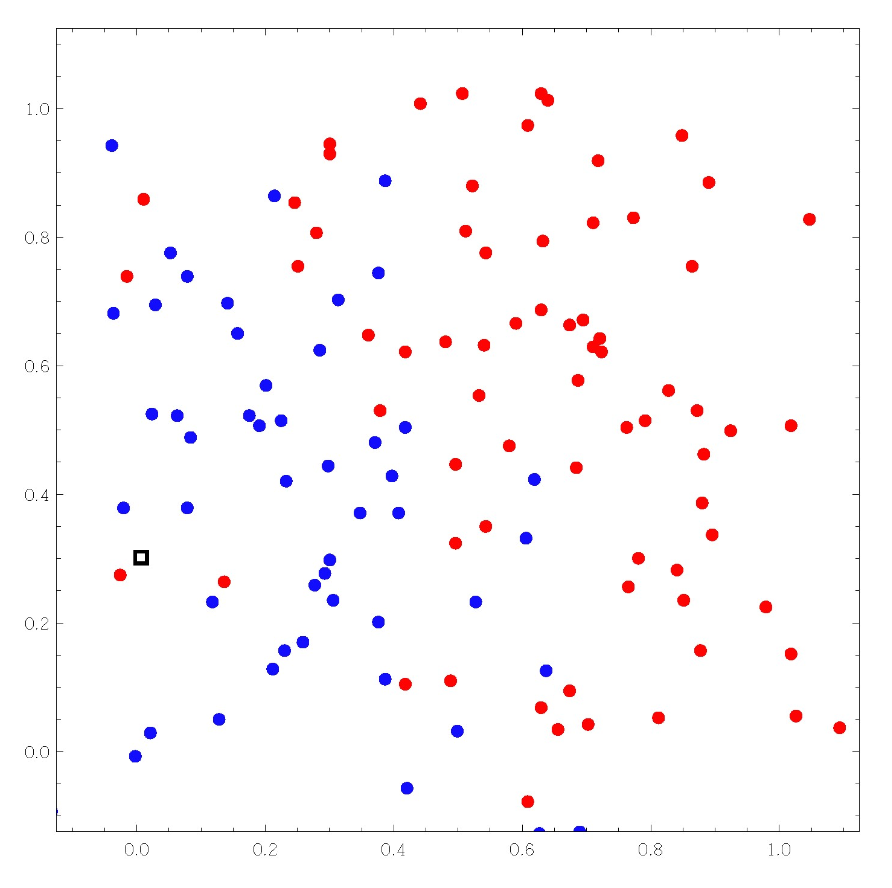
\includegraphics[width=0.7\textwidth]{img/knn.png}
\end{center}

There are $n$ training data points in total and more red points ($y = +1$) than blue points ($y = -1$). A test data point $\mathbf{x}_0$ is shown by a black square, and its label is denoted as $y_0$.

\textbf{Multiple answers are possible!}

\begin{itemize}
    \item[(a)] For $k = 1$: $y_0 = -1$.
    \item[(b)] For $k = 3$: $y_0 = -1$.
    \item[(c)] For $k = n$: $y_0 = -1$.
    \item[(d)] $k = 1$ leads to underfitting.
    \item[(e)] $k = n$ corresponds to large model complexity.
    \item[(f)] In $k$-NN, the parameter $k$ has to be specified before classification.
    \item[(g)] $k$-NN requires use of a distance measure for measuring closeness.
    \item[(h)] $k$-NN can work with labeled and unlabeled data.
\end{itemize}

\subsection*{Bias-variance decomposition for quadratic loss}

Suppose that labels \( y \) for a given feature vector \( \mathbf{x}_0 \) are normally distributed with mean \( \mu = 2 \) and standard deviation \( \sigma = 0.5 \), while the predictions \( g(\mathbf{x}_0; \mathbf{w}(\mathcal{Z}_l)) \) are normally distributed with mean \( \mu = 4 \) and variance \( \sigma^2 = 2.5 \). Compute the expected prediction error for quadratic loss.

\textit{You can use a pocket calculator. Give the answer as a real number, rounded to two decimal places. Use ``.'' for the decimal point. Number format example: 1.23.}

\subsection*{Medical Test Accuracy}

In a group of 50,000 people, 45,000 are healthy, i.e., they are "negative" with respect to a certain disease, and 5,000 are "positive", i.e., they have the disease.

A medical test is developed. The test has a sensitivity of 60\% and a specificity of 80\%. 

What is the accuracy of the test?

\textit{You can use a pocket calculator. Give the answer as a real number between 0 and 1, rounded to two decimal places. Do not give the answer in \%. Use ``.'' for the decimal point. Number format example: 0.67.}

\subsection*{Area Under Curve (AUC) Computation}

Consider the following classification results of a binary classifier tested on 7 samples:

\[
\begin{array}{|c|c|}
\hline
\bar{g}(x) & y \\
\hline
0.1 & 1 \\
-0.8 & -1 \\
1.0 & 1 \\
0.5 & -1 \\
1.9 & -1 \\
-0.1 & -1 \\
1.4 & 1 \\
\hline
\end{array}
\]

Compute the Area Under Curve (AUC) of the ROC curve.

\textit{You can use a pocket calculator. Give the answer as a real number between 0 and 1, rounded to two decimal places. Do not give the answer in \%. Use ``.'' for the decimal point. Number format example: 0.67.}

\subsection*{Support Vector Machines (SVMs)}

Which statements about support vector machines (SVMs) are true? \\
Multiple answers are possible!

\begin{enumerate}[(a)]
    \item Kernels allow to transform data into a lower-dimensional space where separability can easier be achieved.
    \item A sample $\mathbf{x}_i$ is a support vector if the corresponding Lagrange parameter $\alpha_i$ is larger than $0$.
    \item SVMs work effectively if the number of dimensions (features) $d$ is much larger than the number of samples $l$.
    \item For $l$ data points with features $\mathbf{x}_i$, labels $y_i$, and Lagrange parameters $\alpha_i$, the linear SVM classification for a new input $\mathbf{x}$ is given by
          \[
          g(\mathbf{x}) = \text{sign}\left(\sum_{i=1}^l \alpha_i \mathbf{x}_i \cdot \mathbf{x} - b\right).
          \]
    \item One of the KKT conditions has the form: $\alpha_i h_i(\mathbf{w}^*) = 0$ for all $i = 1, \ldots, l$.
    \item The mathematical problem (constrained convex optimization) has a global solution.
    \item Support vector regression uses the magnitude (and not only the sign) of the discriminant function.
    \item SVMs allow for a probabilistic explanation for classification.
\end{enumerate}

\subsection*{Support Vector Machine (SVM) with Linear Kernel}

Consider a C-SVM classifier trained with a linear kernel on a simple 2D dataset (red dots = positive samples, blue dots = negative samples) as depicted below. Blue areas are classified as negative (light blue = inside margin), and red areas are classified as positive (light red = inside margin).

\begin{center}
    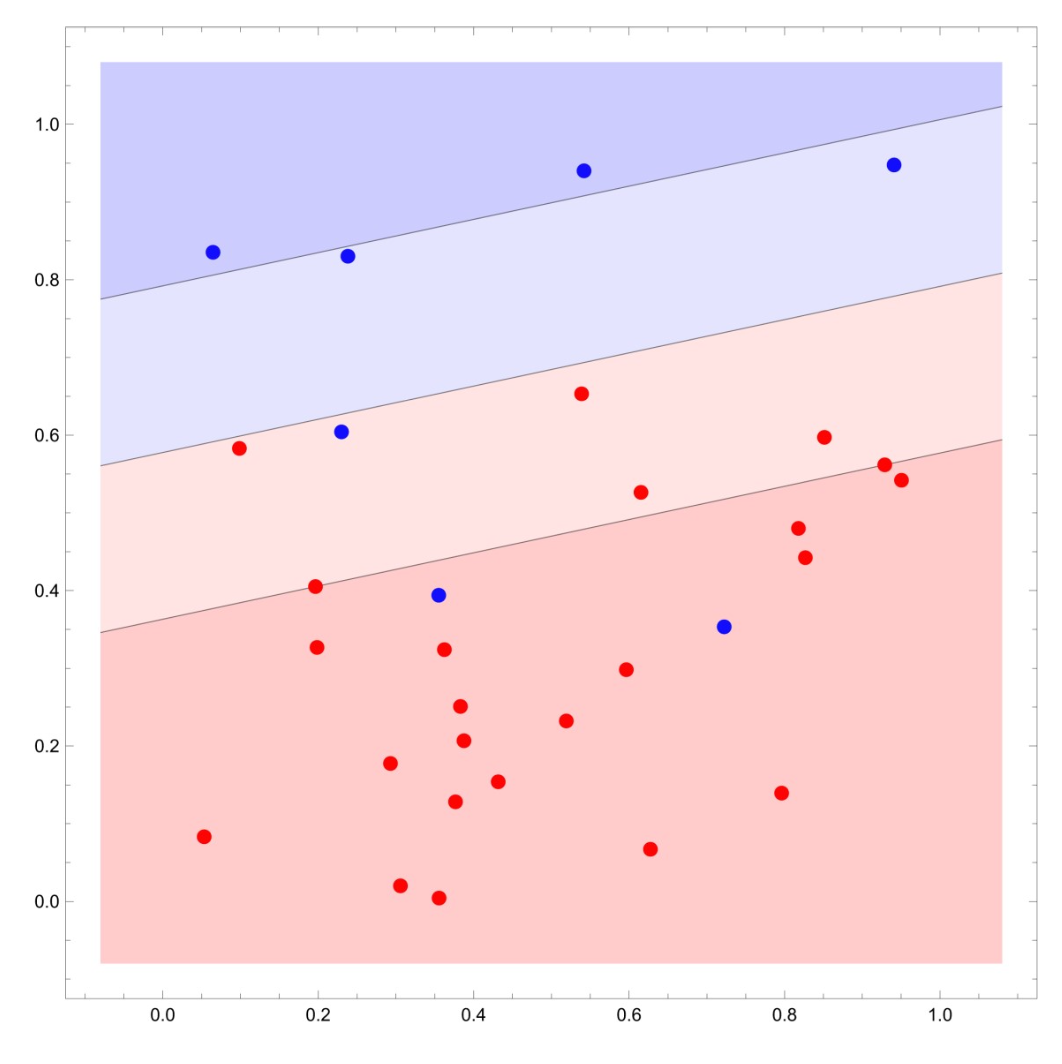
\includegraphics[width=0.7\textwidth]{img/c-svm.png}
\end{center}

Which of the following statements are correct? Multiple answers are possible!

\begin{itemize}
    \item[a)] If the Lagrange multiplier $\alpha_i$ is $0$ for a data point with index $i$, then the slack variable $\xi_i$ must be $0$.
    \item[b)] Just considering the red data points: Exactly $4$ red points are misclassified. They lie inside the margin.
    \item[c)] If the slack variable is larger than $0$ for a data point with index $i$, then also the Lagrange multiplier $\alpha_i$ must be larger than $0$.
    \item[d)] Just considering the blue data points: There are exactly $2$ blue support vectors. They both lie outside the margin in the red territory.
    \item[e)] Considering all data points: Exactly $7$ data points require a slack variable larger than $0$. They lie inside the margin.
\end{itemize}

\subsection*{Multi-Class Classification with Support Vector Machines}

Consider multi-class classification with Support Vector Machines. Let there be \(M\) classes. Which of the following statements are true?

Multiple answers are possible!

\begin{itemize}
    \item[a)] In the one-versus-one approach, there are \(M(M-1)/2\) classifiers.
    \item[b)] In the one-versus-all approach, there are \(M\) classifiers.
    \item[c)] In the one-versus-one approach, the final classification is done by choosing the class which produces the largest value of all classifiers.
    \item[d)] In the one-versus-all approach, the final classification is done by majority vote.
    \item[e)] Training pairwise classifiers is usually more costly due to the larger training sets.
\end{itemize}

\subsection*{Decision Trees}

Which statements about decision trees are true?

Multiple answers are possible!

\begin{itemize}
    \item[a)] Variance reduction is a common splitting criterion for regression.
    \item[b)] Shallow trees tend to underfit, deep trees tend to overfit.
    \item[c)] Decision trees can only be applied to categorical attributes.
    \item[d)] For classification tasks, a new input sample can be assigned to a class value or to a conditional probability.
    \item[e)] The number of leaf nodes cannot be larger than twice the number of internal nodes.
    \item[f)] All decision tree learning algorithms are non-recursive.
    \item[g)] The maximal Gini impurity of a data set with \(M\) classes is \(\ln M\).
    \item[h)] A split maximizes the information gain if the produced subsets are completely homogeneous.
\end{itemize}

\subsection*{Information Gain}

Consider a data set \(\mathbf{Z}\) with 3 different class labels \(y \in \{1, 2, 3\}\). There are \(|\mathbf{Z}| = 1000\) data samples in the set. The probabilities \(p_k\) that a label in the data set belongs to class \(k\) are given as follows:

\[
p_1 = 0.5, \quad p_2 = 0.3, \quad p_3 = 0.2
\]

Assume that a split \(s\) perfectly splits the data set into 3 homogeneous subsets \(\mathbf{Z}_{s,t}\), such that \(\mathbf{Z}_{s,t}\) contains all data samples with label \(t\) (\(t = 1, 2, 3\)).

Let \(H\) denote entropy. Calculate the information gain \(g_E(\mathbf{Z}, s)\):

\[
g_E(\mathbf{Z}, s) = H(\mathbf{Z}) - \sum_{t=1}^3 \frac{|\mathbf{Z}_{s,t}|}{|\mathbf{Z}|} H(\mathbf{Z}_{s,t}).
\]

\textbf{Remark:} In your calculation of the entropy, use the natural logarithm \(\ln = \log_e\), not a logarithm to some other base.

\textbf{Answer:}

You can use a pocket calculator. Give the answer as a real number, rounded to two decimal places. Do not give the answer in \%. Use \texttt{``.''} for the decimal point. Number format example: \texttt{1.67}.

\subsection*{Ensemble Methods: Random Forests and Boosting}

Which statements about ensemble methods, in particular random forests and (gradient) boosting, are true?

\textbf{Multiple answers are possible!}

\begin{itemize}
    \item[(a)] In AdaBoost, the more accurate the weak classifiers are, the larger the influence they are given for the classification output.
    \item[(b)] Random Forests are generally harder to tune compared to Gradient Boosted Trees.
    \item[(c)] Forward stagewise additive modeling is a robust boosting method which specifically depends on the quadratic loss function.
    \item[(d)] A random forest has smaller variance than the individual trees if the correlation between the trees is small.
    \item[(e)] In Boosting, the main idea is that those samples which led to a small error (i.e., were classified well) in an iteration get a larger weight in the next iteration.
    \item[(f)] In general, ensemble methods aim at reducing the bias and increasing the variance.
    \item[(g)] A common measure of variable importance in random forests is the mean accuracy decrease.
    \item[(h)] In a random forest, each individual decision tree is built upon a random bootstrap subsample of the original data set.
\end{itemize}


\subsection*{AdaBoost}

Which statements about AdaBoost are true?

\textbf{Multiple answers are possible!}

\begin{itemize}
    \item[(a)] In every step \(n\), compute a misclassification error and classifier weight \(\alpha_n\). If classification for a data point was correct, leave the corresponding weight unchanged. If classification was wrong, increase the weight.
    \item[(b)] Final output: \(g(\mathbf{x}) = \text{sign} \left( \sum_{n=1}^N \alpha_n \, g_n(\mathbf{x}) \right)\).
    \item[(c)] Initialization: Weights are all initialized to the same value and sum up to 1.
    \item[(d)] In every step, with given weights, find the optimal classifier \(g_n(\mathbf{x})\) to the training data.
\end{itemize}

\subsection*{Logistic Regression and Related Topics}

Which statements about Logistic Regression (and related topics) are true? Multiple answers are possible!

\begin{itemize}
    \item[(a)] In Logistic Regression, minimization of the loss function can be achieved by numerical methods such as gradient descent and conjugate gradient.
    \item[(b)] Assume that \(y\) data are generated around a function \(g(x)\) with Gaussian noise. Minimizing the negative log-likelihood of observing the data is equivalent to minimizing the squared error between \(y\) and \(g(x)\).
    \item[(c)] The logistic (or sigmoid) function reads: \(\sigma(z) = (1 + \exp(-z))^{-1}\).
    \item[(d)] Logistic regression does not have a closed-form solution.
    \item[(e)] The likelihood function for a Bernoulli distribution reads: \(\mathcal{L}(\{\mathbf{x}, \mathbf{y}\}; \mathbf{W}) = \prod_{i=1}^l g(\mathbf{x}_i; \mathbf{W})^{y_i} (1 - g(\mathbf{x}_i; \mathbf{W}))^{1 - y_i}\).
    \item[(f)] The momentum term in gradient descent is particularly helpful in steep regions of the loss function.
    \item[(g)] The softmax function is a generalization of the sigmoid function and is suitable for regression.
    \item[(h)] Logistic Regression is a non-convex problem.
\end{itemize}

\subsection*{Maximum Likelihood}

Assume you have a climate model with an important parameter \(\theta\), namely the level of CO\(_2\) in the atmosphere.

You are given five data points, namely the 10-year-average global temperatures for the past 50 years.

With parameter choice \(\theta_1\), the probabilities to obtain the given data (within a certain margin of error) are: 
\[
\{0.9, 0.9, 0.9, 0.4, 0.9\}.
\]

With parameter choice \(\theta_2\), the probabilities are:
\[
\{0.8, 0.8, 0.75, 0.75, 0.8\}.
\]

Enter numerical values below. You can use a pocket calculator.
\begin{enumerate}[(a)]
    \item How likely is \(\theta_1\) to produce the data? Enter a real number between 0 and 1 rounded to two decimal places. Do not give the answer in \%. Number format example: 0.67
    \item How likely is \(\theta_2\) to produce the data? Enter a real number between 0 and 1 rounded to two decimal places. Do not give the answer in \%. Number format example: 0.67
    \item Which \(\theta_i, i = 1 \text{ or } 2\), is a better explanation for the data? Enter an integer number.
\end{enumerate}

\subsection*{Artificial Neural Networks}

Which statements about Artificial Neural Networks are true? Multiple answers are possible!

\begin{itemize}
    \item[(a)] Dropout and weight decay are regularization techniques which aim at avoiding underfitting.
    \item[(b)] Let us denote the learning rate with \(\eta > 0\), the weights with \(\mathbf{w}\), and the empirical risk with \(\mathbf{R}\). Then the gradient descent update rule reads: 
    \[
    \mathbf{w}_{\text{new}} = \mathbf{w}_{\text{old}} + \eta \nabla_{\mathbf{w}} \mathbf{R}.
    \]
    \item[(c)] Using the matrix-vector notation from the lecture (Unit 6), the recursive formula for delta errors is given by:
    \[
    \delta^{[l-1]^T} = \delta^{[l]^T} \mathbf{J}^{[l]}.
    \]
    Here, \(\mathbf{J}^{[l]}\) is the single-layer Jacobian for layer \(l\).
    \item[(d)] Multi-layer perceptrons are equivalent to fully connected feed-forward neural networks.
    \item[(e)] The vanishing gradient problem can be mitigated/avoided by the use of suitable activation functions.
    \item[(f)] The perceptron is a simple non-linear classifier.
    \item[(g)] The Universal Approximation Theorem guarantees that neural networks have small VC dimension.
    \item[(h)] Without activation functions, neural networks are linear functions with respect to their weights.
\end{itemize}

\subsection*{Perceptrons and Perceptron Learning}

Which statements about Perceptrons and Perceptron Learning are true? Multiple answers are possible!

\textbf{Notation as in the lecture:}
\begin{itemize}
    \item Weight vector: \(\mathbf{w}\)
    \item Threshold: \(\theta\)
    \item Data samples: \(\mathbf{x}_i\)
    \item Learning rate: \(\eta > 0\)
\end{itemize}

\begin{itemize}
    \item[(a)] If the data set is linearly separable, then there exists a stopping criterion such that with probability 1 the perceptron learning algorithm will terminate and solve the learning task.
    \item[(b)] In the learning algorithm: If \(g(\mathbf{x}_i; \mathbf{w}, \theta) = 1\) and \(y_i = 0\), then the update rule for the threshold reads: 
    \[
    \theta := \theta + \eta.
    \]
    \item[(c)] The perceptron is a non-linear classifier.
    \item[(d)] The final solution (values of the \(\mathbf{w}\) and \(\theta\)) of the perceptron learning algorithm may depend on the initialization.
    \item[(e)] A perceptron can solve the XOR problem, but only in certain instances, and then the solution is not unique.
    \item[(f)] In the learning algorithm: If \(g(\mathbf{x}_i; \mathbf{w}, \theta) = 0\) and \(y_i = 1\), then the update rule for the weight vector reads:
    \[
    \mathbf{w} := \mathbf{w} - \eta \mathbf{x}_i.
    \]
\end{itemize}

\subsection*{Convolutional Neural Networks (CNNs)}

Which statements are true? Multiple answers are possible!

\begin{itemize}
    \item[(a)] Dataset augmentation can help to overcome the problem of limited quantity and/or diversity of given data.
    \item[(b)] With kernel weight matrix \(w_{i,j}\), kernel size \(R\), and input image \(x_{a,b}\), the feature map preactivation is calculated by:
    \[
    s_{a,b} = \sum_{i=0}^{R-1} \sum_{j=0}^{R-1} w_{i,j} x_{a,b}.
    \]
    \item[(c)] With input dimension \(A\), kernel size \(R\), padding \(P\), and stride \(S\), the feature map dimension is:
    \[
    \frac{A + R + 2P}{S} + 1.
    \]
    \item[(d)] Re-using a kernel weight matrix at all positions of an image is called weight sharing.
    \item[(e)] A convolutional layer can use multiple kernels.
    \item[(f)] ResNet is a famous CNN, whose good learning performance is due to skip connections.
    \item[(g)] Transfer Learning allows to use a kernel from one convolutional layer also in the next (neighbouring) layer.
    \item[(h)] Pooling increases the receptive field through the depth of the network.
\end{itemize}

\subsection*{Convolution}

You are given the input image \(\mathbf{x}\) with two channels:

\[
\mathbf{x}_{c=1} =
\begin{bmatrix}
2 & 1 & 2 & 0 & 1 & 0 & 1 \\
1 & 1 & 1 & 1 & 1 & 1 & 1 \\
2 & 0 & 1 & 2 & 0 & 1 & 2 \\
0 & 0 & 0 & 0 & 0 & 0 & 0 \\
2 & 2 & 2 & 2 & 2 & 2 & 2 \\
1 & 2 & 2 & 2 & 1 & 2 & 1
\end{bmatrix},
\quad
\mathbf{x}_{c=2} =
\begin{bmatrix}
1 & 1 & 1 & 0 & 0 & 2 & 2 \\
1 & 1 & 0 & 1 & 2 & 2 & 0 \\
0 & 1 & 2 & 0 & 1 & 0 & 1 \\
0 & 0 & 1 & 2 & 0 & 1 & 0 \\
2 & 0 & 0 & 2 & 0 & 2 & 0 \\
1 & 2 & 2 & 0 & 1 & 2 & 0
\end{bmatrix}.
\]

The filter \(\mathbf{W}\) with depth 2 is given by:

\[
\mathbf{W}_{c=1} =
\begin{bmatrix}
0 & 1 & 0 \\
1 & -4 & 1 \\
0 & 1 & 0
\end{bmatrix},
\quad
\mathbf{W}_{c=2} =
\begin{bmatrix}
1 & 0 & -1 \\
0 & 0 & 0 \\
-1 & 0 & 1
\end{bmatrix}.
\]

\begin{enumerate}[(a)]
    \item Assuming stride equal to 1 and no padding, compute the top-right entry \(s_{1,5}\) of the preactivation \(\mathbf{s} = \mathbf{W} * \mathbf{x}\) by convolution (cross-correlation, to be precise).
    \item Assuming no padding and stride equal to 2, the dimension of the output matrix becomes \(d \times d\). Compute \(d\).
    \item Assuming padding equal to 1 and stride equal to 3, the dimension of the output matrix becomes \(D \times D\). Compute \(D\).
\end{enumerate}

\textbf{Answers:}
\begin{itemize}
    \item \(s_{1,5} =\)
    \item \(d = \)
    \item \(D = \)
\end{itemize}

\subsection*{Recurrent Neural Networks (RNNs)}

Which statements about Recurrent Neural Networks (RNNs) are true? Multiple answers are possible!

\begin{itemize}
    \item[(a)] In an RNN, the units in a hidden layer are all connected with each other but cannot be connected to themselves.
    \item[(b)] The constant error carousel in LSTMs must use a non-linear activation function in order to avoid the vanishing gradient problem.
    \item[(c)] RNNs can be trained via Backpropagation Through Time.
    \item[(d)] We denote with \(\mathbf{R}\) the recurrent weight matrix at time \(t\), with \(f\) the activation function, and with \(\mathbf{s}(t-1)\) the preactivation at time \(t-1\). For stable gradients, we need \(\|\mathbf{R} \, \text{diag}(f(\mathbf{s}(t-1)))\| \approx 1\).
    \item[(e)] Feedforward neural networks (FNNs) are Turing complete.
    \item[(f)] LSTMs use an integrator to store information and gates for remembering, communicating, and (potentially) forgetting.
    \item[(g)] RNNs use weight sharing as the network is slid over the input sequence and the hidden-layer weight matrix is reused for all timesteps.
    \item[(h)] RNNs are typically useful for sequence classification and generation.
\end{itemize}

\subsection*{Generalization Error and Empirical Risk}

Which statements about the generalization error and the empirical risk are true?

\textbf{Multiple answers are possible!}

\begin{itemize}
    \item[(a)] The generalization error is the expected loss on future data for a given model.
    \item[(b)] The generalization error has the form:
    \[
    \int_X \int_{\mathbb{R}} L(y, g(\vec{x}; \vec{w})) p(\vec{x} \mid y) p(y) \, d\vec{x} \, dy.
    \]
    \item[(c)] The empirical risk on a dataset with \(n\) samples has the form:
    \[
    R_{\text{emp}} = \frac{1}{n} \prod_{i=1}^n L(y_i, g(\vec{x}_i; \vec{w})).
    \]
    \item[(d)] A common assumption for estimation of the generalization error via the empirical risk is that data are independent and identically distributed (i.i.d.).
    \item[(e)] A good estimation of the generalization error via the empirical risk generally requires that data points are uniformly distributed.
    \item[(f)] A good estimation of the generalization error via the empirical risk generally requires a large number of samples.
    \item[(g)] A good estimation of the generalization error via the empirical risk generally requires use of a differentiable loss function.
    \item[(h)] Estimating the risk via samples from a test set, which have not been used in training, avoids the problem of underfitting.
\end{itemize}

\subsection*{Bias Variance Decomposition for Quadratic Loss}

Suppose that labels \(y\) for a given feature vector \(\mathbf{x}_0\) are normally distributed with mean \(\mu = 2\) and standard deviation \(\sigma = 0.5\), while the predictions \(g(\mathbf{x}_0; \mathbf{w}(\mathcal{Z}_l))\) are normally distributed with mean \(\mu = 4\) and variance \(\sigma^2 = 2.5\). Compute the expected prediction error for quadratic loss.

\textit{You can use a pocket calculator. Give the answer as a real number, rounded to two decimal places. Use ``.'' for the decimal point. Number format example: 1.23.}

\textbf{Answer:}

\subsection*{Medical Test Accuracy}

In a group of 50,000 people, 45,000 are healthy, i.e., they are "negative" with respect to a certain disease, and 5,000 are "positive", i.e., they have the disease.

A medical test is developed. The test has a sensitivity of 60\% and a specificity of 80\%.

What is the accuracy of the test?

\textit{You can use a pocket calculator. Give the answer as a real number between 0 and 1, rounded to two decimal places. Do not give the answer in \%. Use ``.'' for the decimal point. Number format example: 0.67.}

\subsection*{Area Under Curve (AUC) Computation}

Consider the following classification results of a binary classifier tested on 7 samples:

\[
\begin{array}{|c|c|}
\hline
\bar{g}(x) & y \\
\hline
0.1 & 1 \\
-0.8 & -1 \\
1.0 & -1 \\
0.5 & -1 \\
1.9 & 1 \\
-0.1 & -1 \\
1.4 & 1 \\
\hline
\end{array}
\]

Compute the Area Under Curve (AUC) of the ROC curve.

\textit{You can use a pocket calculator. Give the answer as a real number between 0 and 1, rounded to two decimal places. Do not give the answer in \%. Use ``.'' for the decimal point. Number format example: 0.67.}

\subsection*{Supervised Machine Learning}

Which statements about supervised machine learning are true?

\textbf{Multiple answers are possible!}

\begin{itemize}
    \item[(a)] The Bayes Optimal Classifier is a probabilistic model that makes the most probable prediction for a new sample.
    \item[(b)] Supervised machine learning uses data with supervisory signals for predictive modeling.
    \item[(c)] ROC curves allow to evaluate a classifier independent of class distribution and independent of misclassification cost.
    \item[(d)] Bias increases with increasing model class complexity.
    \item[(e)] Having a small training error but a large test error indicates overfitting.
    \item[(f)] Model variance decreases with increasing model class complexity.
    \item[(g)] Supervised machine learning uses explicit knowledge to design models deductively.
    \item[(h)] The more degrees of freedom, the lower the risk to fit to noise.
\end{itemize}

\subsection*{Support Vector Machines (SVMs)}

Which statements about support vector machines (SVMs) are true?

\textbf{Multiple answers are possible!}

\begin{itemize}
    \item[(a)] SVMs work effectively if the number of dimensions (features) \(d\) is much smaller than the number of samples \(l\).
    \item[(b)] SVMs allow for a probabilistic explanation for classification.
    \item[(c)] The Gaussian kernel has the form:
    \[
    k(\mathbf{x}_i, \mathbf{x}_j) = \exp\left(-\frac{1}{2\sigma^2} \|\mathbf{x}_i - \mathbf{x}_j\|^2 \right).
    \]
    \item[(d)] One of the KKT conditions has the form:
    \[
    \alpha_i h_i(\mathbf{w}^*) \geq 0 \quad \text{for all } i = 1, \ldots, l.
    \]
    \item[(e)] A sample \(\mathbf{x}_i\) is a support vector if and only if the corresponding Lagrange parameter \(\alpha_i\) is strictly larger than 0.
    \item[(f)] Support vector regression uses the magnitude (and not only the sign) of the discriminant function.
    \item[(g)] The mathematical problem (constrained convex optimization) has a global solution.
    \item[(h)] Kernels allow to transform data into a lower-dimensional space where separability can be easier achieved.
\end{itemize}

\subsection*{Constrained Optimization Problem}

Find the solution \(\hat{w}_1, \hat{w}_2\) to the following constrained optimization problem with respect to \(w_1, w_2\):

\[
\text{minimize} \quad \frac{1}{2}(w_1^2 + w_2^2)
\]
\[
\text{subject to} \quad 3 - w_1 - 2w_2 \leq 0.
\]

You can use a pocket calculator. Give the answer as a real number, rounded to one decimal place. Use ``.'' or ``,'' for the decimal point (depending on what works with your system). Number format example: 2.1 or 2,1.

\begin{itemize}
    \item \(\hat{w}_1 = \)
    \item \(\hat{w}_2 = \)
\end{itemize}

\subsection*{Dual Problem Formulation}

Consider the primal problem:

\[
\text{Minimization of } f(\mathbf{w}) \quad \text{subject to } h_i(\mathbf{w}) \leq 0 \text{ for } i = 1, \ldots, l
\]

The Lagrange function reads:
\[
L(\mathbf{w}; \alpha_1, \ldots, \alpha_l) = f(\mathbf{w}) + \sum_{i=1}^l \alpha_i h_i(\mathbf{w}) \quad \text{where } \alpha_i \text{ are Lagrange multipliers.}
\]

What is the corresponding dual problem?

\begin{enumerate}[(a)]
    \item Maximize \(L(\mathbf{w}; \alpha_1, \ldots, \alpha_l)\) w.r.t. \(\alpha_1, \ldots, \alpha_l\), subject to \(\alpha_i \geq 0 \text{ for } i = 1, \ldots, l\)
    \item Minimize \(L(\mathbf{w}; \alpha_1, \ldots, \alpha_l)\) w.r.t. \(\alpha_1, \ldots, \alpha_l\), subject to \(\alpha_i \geq 0 \text{ for } i = 1, \ldots, l\)
    \item Maximize \(L(\mathbf{w}; \alpha_1, \ldots, \alpha_l)\) w.r.t. \(\mathbf{w}\), subject to \(\alpha_i \geq 0 \text{ for } i = 1, \ldots, l\)
    \item Minimize \(L(\mathbf{w}; \alpha_1, \ldots, \alpha_l)\) w.r.t. \(\mathbf{w}\), subject to \(\alpha_i \geq 0 \text{ for } i = 1, \ldots, l\)
    \item Maximize \(\inf_{\mathbf{w}} L(\mathbf{w}; \alpha_1, \ldots, \alpha_l)\) w.r.t. \(\alpha_1, \ldots, \alpha_l\), subject to \(\alpha_i \geq 0 \text{ for } i = 1, \ldots, l\)
    \item Minimize \(\inf_{\mathbf{w}} L(\mathbf{w}; \alpha_1, \ldots, \alpha_l)\) w.r.t. \(\alpha_1, \ldots, \alpha_l\), subject to \(\alpha_i \geq 0 \text{ for } i = 1, \ldots, l\)
    \item Maximize \(\inf_{\alpha_1, \ldots, \alpha_l} L(\mathbf{w}; \alpha_1, \ldots, \alpha_l)\) w.r.t. \(\mathbf{w}\), subject to \(\alpha_i \geq 0 \text{ for } i = 1, \ldots, l\)
    \item Minimize \(\inf_{\mathbf{w}} L(\mathbf{w}; \alpha_1, \ldots, \alpha_l)\) w.r.t. \(\mathbf{w}\), subject to \(\alpha_i \geq 0 \text{ for } i = 1, \ldots, l\)
\end{enumerate}

\subsection*{Support Vectors in SVM}

Consider a C-SVM classifier trained with a linear kernel on a simple 2D dataset (red dots = positive samples, blue dots = negative samples) as depicted below. Blue areas are classified as negative (light blue = inside margin), and red areas are classified as positive (light red = inside margin).

\textbf{How many support vectors are there?}

\begin{center}
    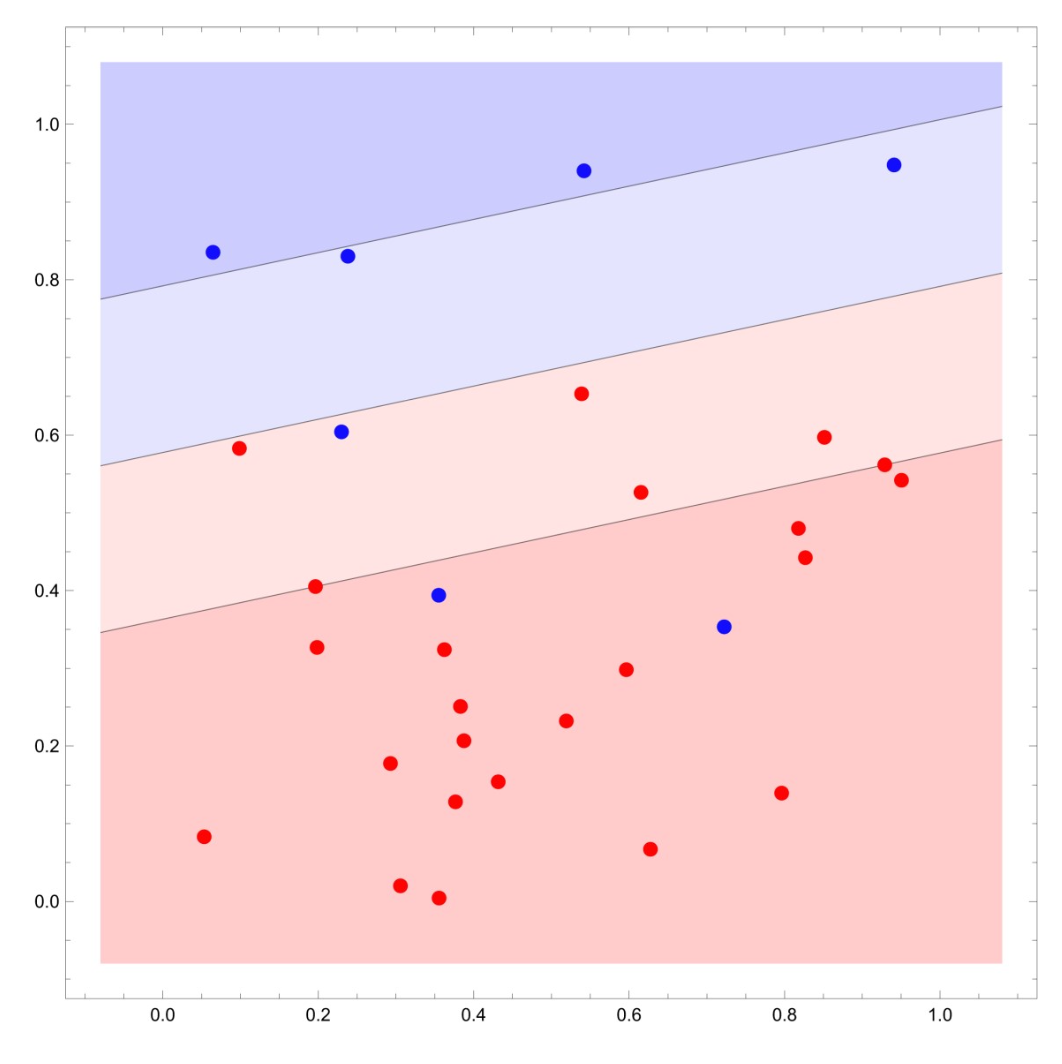
\includegraphics[width=0.7\textwidth]{img/c-svm.png}
\end{center}

\textbf{Choose one answer:}

\begin{itemize}
    \item[(a)] 0
    \item[(b)] 1
    \item[(c)] 2
    \item[(d)] 3
    \item[(e)] 4
    \item[(f)] 5
    \item[(g)] 6
    \item[(h)] 7
    \item[(i)] 8
    \item[(j)] 9
    \item[(k)] More than 9
\end{itemize}

\subsection*{Multi-Class Classification with Support Vector Machines}

Consider multi-class classification with Support Vector Machines. Let there be \(M\) classes. Which of the following statements are true?

\textbf{Multiple answers are requested!}

\begin{enumerate}[(a)]
    \item In the one-versus-one approach, there are \(M - 1\) classifiers.
    \item In the one-versus-one approach, there are \(M\) classifiers.
    \item In the one-versus-one approach, there are \(\frac{M(M-1)}{2}\) classifiers.
    \item In the one-versus-one approach, there are \(\frac{M(M+1)}{2}\) classifiers.
    \item In the one-versus-all approach, there are \(M - 1\) classifiers.
    \item In the one-versus-all approach, there are \(M\) classifiers.
    \item In the one-versus-all approach, there are \(\frac{M(M-1)}{2}\) classifiers.
    \item In the one-versus-all approach, there are \(\frac{M(M+1)}{2}\) classifiers.
    \item In the one-versus-one approach, the final classification is done by choosing the class which produces the largest value of all classifiers.
    \item In the one-versus-one approach, the final classification is done by majority vote.
    \item In the one-versus-all approach, the final classification is done by choosing the class which produces the largest value of all classifiers.
    \item In the one-versus-all approach, the final classification is done by majority vote.
\end{enumerate}

\subsection*{Decision Trees}

Which statements about decision trees are true?

\textbf{Multiple answers are possible!}

\begin{enumerate}[(a)]
    \item Variance reduction is a common splitting criterion for regression.
    \item The number of leaf nodes cannot be larger than twice the number of internal nodes.
    \item All decision tree learning algorithms are non-recursive.
    \item For classification tasks, a new input sample can be assigned to a class value or to a conditional probability.
    \item A split maximizes the information gain if the produced subsets are completely homogeneous.
    \item The maximal Gini impurity of a data set with \(M\) classes is \(\ln M\).
    \item Decision trees can only be applied to categorical attributes.
    \item Shallow trees tend to underfit, deep trees tend to overfit.
\end{enumerate}

\subsection*{Information Gain Calculation}

Consider a data set \(\mathbf{Z}\) with 3 different class labels \(y \in \{1, 2, 3\}\). There are \(|\mathbf{Z}| = 1000\) data samples in the set. The probabilities \(p_k\) that a label in the data set belongs to class \(k\) are given as follows:

\[
p_1 = 0.5, \quad p_2 = 0.3, \quad p_3 = 0.2
\]

Assume that a split \(s\) perfectly splits the data set into 3 homogeneous subsets \(\mathbf{Z}_{s,t}\), such that \(\mathbf{Z}_{s,t}\) contains all data samples with label \(t\) (\(t = 1, 2, 3\)).

Let \(H\) denote entropy. Calculate the information gain \(g_E(\mathbf{Z}, s)\):

\[
g_E(\mathbf{Z}, s) = H(\mathbf{Z}) - \sum_{t=1}^3 \frac{|\mathbf{Z}_{s,t}|}{|\mathbf{Z}|} H(\mathbf{Z}_{s,t}).
\]

\textbf{Remark:} In your calculation of the entropy, use the natural logarithm \(\ln\), not a logarithm to some other base.

\textbf{Answer:} \texttt{1.03}

\textit{You can use a pocket calculator. Give the answer as a real number, rounded to two decimal places. Do not give the answer in \%. Use \texttt{"."} for the decimal point. Number format example: \texttt{1.67}.}

\subsection*{Random Forests and Boosting}

Which statements about ensemble methods, in particular random forests and (gradient) boosting, are true?

\textbf{Multiple answers are possible!}

\begin{enumerate}[(a)]
    \item In general, ensemble methods aim at reducing the bias and increasing the variance.
    \item Gradient Boosted Trees are generally much easier to tune compared to Random Forests.
    \item A random forest in general has smaller bias than the individual trees.
    \item Forward stagewise additive modelling is a robust boosting method which can be applied to different loss functions.
    \item In AdaBoost, the more accurate the weak classifiers are, the higher the influence they are given for the classification output.
    \item In a random forest, each individual decision tree is built upon a random bootstrap subsample of the original data set.
    \item In Boosting, the main idea is that those samples which led to a small error (i.e., were classified well) in an iteration get a larger weight in the next iteration.
    \item A common measure of variable importance in random forests is the mean decrease in Gini impurity.
\end{enumerate}

\subsection*{Logistic Regression (and Related Topics)}

Which statements about Logistic Regression (and related topics) are true?

\textbf{Multiple answers are possible!}

\begin{enumerate}[(a)]
    \item Logistic Regression is a convex problem.
    \item The logistic function reads: 
    \[
    \sigma(z) = (1 + \exp(-z))^{-1}.
    \]
    It is also known as the sigmoid function.
    \item The likelihood function for a Bernoulli distribution reads:
    \[
    \mathcal{L}(\{\mathbf{x}, \mathbf{y}\}; \mathbf{W}) = \prod_{i=1}^l g(\mathbf{x}_i; \mathbf{W})^{y_i} (1 - g(\mathbf{x}_i; \mathbf{W}))^{1 - y_i}.
    \]
    \item The softmax function is a generalization of the sigmoid function and is suitable for multi-class classification.
    \item In Logistic Regression, minimization of the loss function can be achieved by gradient descent.
    \item The momentum term in gradient descent is particularly helpful in steep regions of the loss function.
    \item Assume that \(y\) data are generated around a function \(g(x)\) with Gaussian noise. Minimizing the negative log-likelihood of observing the data is equivalent to maximizing the squared error between \(y\) and \(g(x)\).
    \item Logistic regression has a closed-form solution.
\end{enumerate}

\subsection*{Maximum Likelihood}

Assume you have a climate model with an important parameter \(\theta\), namely the level of CO\(_2\) in the atmosphere.

You are given five data points, namely the 10-year-average global temperatures for the past 50 years.

With parameter choice \(\theta_1\), the probabilities to obtain the given data within a certain margin of error are:
\[
\{0.8, 0.9, 0.9, 0.7, 0.8\}.
\]

With parameter choice \(\theta_2\), the probabilities are:
\[
\{0.9, 0.9, 0.5, 0.9, 0.9\}.
\]

\begin{enumerate}
    \item How likely is \(\theta_1\) to produce the data?
    \item How likely is \(\theta_2\) to produce the data?
\end{enumerate}

Enter numerical values below. You can use a pocket calculator. Enter real numbers between 0 and 1 rounded to two decimal places. Do not give the answer in \%. Number format example: 0.67.

\begin{itemize}
    \item \(\mathcal{L}(\theta_1) =\)
    \item \(\mathcal{L}(\theta_2) =\)
\end{itemize}

\subsection*{Logistic Regression}

You are given the feature vector \(\mathbf{x} = (1, 2, 3, 4, 5)\) and the weight vector \(\mathbf{W} = (1, -1, 1, -1, 1)\).

What is the output of a logistic regression model? (Enter your real-valued result; do not apply the sign function.)

You can use a pocket calculator. Give the answer as a real number, rounded to two decimal places. Use "." for the decimal point. Number format example: 1.23.

\textbf{Answer:}

\subsection*{Artificial Neural Networks}

Which statements about Artificial Neural Networks are true?

Multiple answers are possible!

\begin{enumerate}[(a)]
    \item Without activation functions, neural networks are linear functions with respect to their weights.
    \item Dropout and weight decay are regularization techniques which aim at avoiding underfitting.
    \item Multi-layer perceptrons are equivalent to fully connected feed-forward neural networks.
    \item The vanishing gradient problem can be mitigated/avoided by the use of suitable activation functions.
    \item Let us denote the learning rate with \(\eta > 0\), the weights with \(\mathbf{w}\), and the empirical risk with \(\mathcal{R}\). Then the gradient descent update rule reads:
    \[
    \mathbf{w}_{\text{new}} = \mathbf{w}_{\text{old}} + \eta \nabla_{\mathbf{w}} \mathcal{R}.
    \]
    \item The perceptron is a simple non-linear classifier.
    \item Using the matrix-vector notation from the lecture (Unit 6), the recursive formula for delta errors is given by:
    \[
    \delta^{[l-1]T} = \delta^{[l]T} \mathbf{J}^{[l]}.
    \]
    Here, \(\mathbf{J}^{[l]}\) is the single-layer Jacobian for layer \(l\).
    \item The Universal Approximation Theorem guarantees that neural networks have small VC dimension.
\end{enumerate}

\subsection*{Jacobian Calculation}

The single-layer Jacobian reads:
\[
\mathbf{J}^{[l]} = \mathbf{W}^{[l]} \operatorname{diag}\left(f'(s^{[l-1]})\right).
\]

Assume that the preactivation vector is given by:
\[
s^{[l-1]} = \begin{pmatrix} -3 \\ -1 \\ 2 \end{pmatrix}.
\]

As the activation function \(f\), take the ReLU function.

The weight matrix is:
\[
\mathbf{W}^{[l]} = \begin{pmatrix}
1 & 2 & 3 \\
4 & 5 & 6 \\
7 & 8 & 9
\end{pmatrix}.
\]

Compute the bottom right entry of the Jacobian \(\mathbf{J}^{[l]}_{3,3}\).

\textbf{The answer is an integer number.}

\subsection*{Convolutional Neural Networks (CNNs):}

\textbf{Which statements are true?}

\textit{Multiple answers are possible!}

\begin{enumerate}[(a)]
    \item Re-using a kernel weight matrix multiple positions of an image is called weight sharing.
    \item Transfer Learning allows to use pretrained kernels from other networks which were trained on different data sets.
    \item With input dimension \(A\), kernel size \(R\), padding \(P\), and stride \(S\), the feature map dimension is 
    \[
    \frac{(A + R + 2P)}{S} + 1.
    \]
    \item With kernel weight matrix \(w_{i,j}\), kernel size \(R\), and input image \(x_{a,b}\), the feature map preactivation is calculated by 
    \[
    s_{a,b} = \sum_{i=0}^{R-1} \sum_{j=0}^{R-1} w_{i,j} \, x_{a+i, b+j}.
    \]
    \item Each convolutional layer always uses exactly one kernel.
    \item AlexNet is a famous CNN, whose good learning performance is due to skip connections.
    \item Dataset augmentation can help to overcome the problem of limited quantity and/or diversity of given data.
    \item Pooling decreases the receptive field through the depth of the network.
\end{enumerate}

\subsection*{Recurrent Neural Networks (RNNs):}

\textbf{Which statements are true?}

\textit{Multiple answers are possible!}

\begin{enumerate}[(a)]
    \item RNNs use weight sharing as the network is slid over the input sequence and the hidden-layer weight matrix is reused for all timesteps.
    \item In an RNN, the units in a hidden layer are all connected with each other but cannot be connected to themselves.
    \item The operations complexity of backpropagation through time for an RNN with \(N\) hidden units and sequence length \(T\) is \(\mathcal{O}(N^2 T)\).
    \item LSTMs use an integrator to store information and gates for remembering, communicating, and (potentially) forgetting.
    \item The constant error carousel in LSTMs must use a non-linear activation function in order to avoid the vanishing gradient problem.
    \item Feedforward neural networks (FNNs) are Turing complete.
    \item We denote with \(\mathbf{R}(t)\) the recurrent weight matrix at time \(t\), with \(f\) the activation function, and with \(\mathbf{s}(t-1)\) the preactivation at time \(t-1\). For stable gradients, we need 
    \[
    \|\mathbf{R}(t) \, \text{diag}(f'(\mathbf{s}(t-1)))\| \approx 1.
    \]
    \item RNNs are typically useful for sequence classification and generation.
\end{enumerate}

\subsection*{Constrained Optimization Problem:}

\textbf{Find the solution \((w_1^*, w_2^*)\) to the following constrained optimization problem and enter \(w_1^*\) in the field below:}

\[
f(w_1, w_2) = 1w_1^2 + w_2^2
\]
\[
h(w_1, w_2) = 2w_1 + w_2 - 7 \leq 0.
\]

You can use a pocket calculator. Give the answer as a real number, rounded to two decimal places. Use ``.'' or ``,'' for the decimal point (depending on what works with your system). Number format example: 2.14 or 2,14. If the answer is an integer, still add the decimal point and trailing zeros such that it has two decimal places, for example: 2.00 or 2,00.

\textbf{Answer:}

\subsection*{Gini Purity Gain}

\textbf{Problem:}

Consider the result of training a decision tree which partitions the depicted binary data (classes: \(+\) and \(-\)) into three regions.

\begin{center}
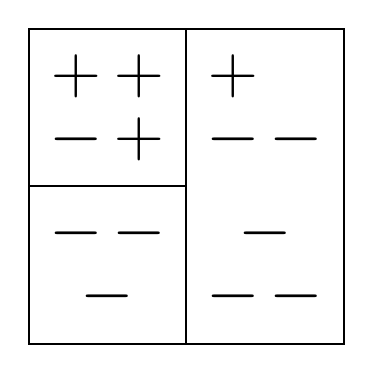
\begin{tikzpicture}[scale=2]
    % Draw the main rectangle
    \draw[thick] (0, 0) rectangle (2, 2);

    % Draw the partitions
    \draw[thick] (1, 0) -- (1, 2); % Vertical line
    \draw[thick] (0, 1) -- (1, 1); % Horizontal line on the left

    % Top-left region
    \node at (0.3, 1.7) {\Huge$+$};
    \node at (0.7, 1.7) {\Huge$+$};
    \node at (0.7, 1.3) {\Huge$+$};
    \node at (0.3, 1.3) {\Huge$-$};

    % Bottom-left region
    \node at (0.3, 0.7) {\Huge$-$};
    \node at (0.7, 0.7) {\Huge$-$};
    \node at (0.5, 0.3) {\Huge$-$};

    % Right region
    \node at (1.3, 1.7) {\Huge$+$};
    \node at (1.7, 1.3) {\Huge$-$};
    \node at (1.3, 1.3) {\Huge$-$};
    \node at (1.5, 0.7) {\Huge$-$};
    \node at (1.3, 0.3) {\Huge$-$};
    \node at (1.7, 0.3) {\Huge$-$};
\end{tikzpicture}
\end{center}
\[
\text{What is the Gini purity gain of the resulting partition?}
\]

\textbf{Instructions:}

You can use a pocket calculator. Give the answer as a real number between 0 and 1, rounded to two decimal places. Do not give the answer in \%. Use ``.'' for the decimal point. Number format example: 0.67.

\textbf{Answer:}



\subsection*{Threshold Model and Cross-Validation}

Consider the following dataset which is already split into three folds:

\[
\begin{array}{|c|c|c|c|c|c|c|}
\hline
 & \multicolumn{2}{c|}{\textbf{F1}} & \multicolumn{2}{c|}{\textbf{F2}} & \multicolumn{2}{c|}{\textbf{F3}} \\ \hline
\textbf{x} & 5 & 2 & 0 & 7 & -1 & -5 \\ \hline
\textbf{y} & 1 & -1 & -1 & 1 & 1 & 1 \\ \hline
\end{array}
\]



Assume that you want to train a threshold model \( g(x, w) \) with parameter \( w \) given by:

\[
g(x, w) =
\begin{cases} 
+1 & \text{if } x \geq w, \\
-1 & \text{else}.
\end{cases}
\]

Given a training set \(\{(x_i, y_i)\}_{i=1}^l\), \( w \) is determined by the average sum of absolute error on these data, i.e.,
\[
w = \frac{1}{l} \sum_{i=1}^l |x_i - y_i|.
\]

In order to estimate the generalization error with cross-validation, solve the following tasks:
\begin{enumerate}
    \item What is the resulting parameter \( w \), if the first fold is considered for evaluation? \textbf{Answer:} \_\_\_\_\_\_
    \item What is the resulting risk for the 1st fold, i.e., \( L_{cv,1} \), if the 0-1-loss is used as loss function? \textbf{Answer:} \_\_\_\_\_\_
\end{enumerate}

\textit{You can use a pocket calculator. Give the answer as a real number between 0 and 1, rounded to two decimal places. Do not give the answer in \%. Use \texttt{"."} for the decimal point. Number format example: \texttt{0.67}.}



\subsection*{Area Under Curve (AUC) and Threshold for ROC Curve}

Consider the following result of a model \( g \) for a binary classification task. \( y \) denotes the true labels.

\[
\begin{array}{|c|c|}
\hline
\bar{g}(x) & y \\ \hline
0.01 & 1.0 \\ \hline
0.44 & 1.0 \\ \hline
0.66 & -1.0 \\ \hline
0.83 & 1.0 \\ \hline
0.91 & 1.0 \\ \hline
-0.55 & -1.0 \\ \hline
-0.33 & -1.0 \\ \hline
-0.13 & -1.0 \\ \hline
\end{array}
\]

\begin{itemize}
    \item \textbf{Task 1:} Calculate the Area Under Curve (AUC) of the associated ROC-curve.
    \item \textbf{Task 2:} Identify which part of the ROC-curve corresponds to the threshold \(\theta = 0.1\) for the associated threshold model \(\bar{g}(x) = \text{sgn}(g(x) - \theta)\). Specify the False Positive Rate (FPR) and True Positive Rate (TPR).
\end{itemize}

\textit{You can use a pocket calculator. Give your answers as real numbers between 0 and 1, rounded to two decimal places. Do not give the answer in \%. Use \texttt{"."} for the decimal point. Number format example: \texttt{0.67}.}

\subsection*{Bias, Variance, and Prediction Error}

Similar to what you saw in the lecture, consider the following data points and model distributions.

The vertical axis is the \(y\)-axis (corresponding to the labels), the horizontal axis is the \(x\)-axis of a single feature. The green lines are different trained models. The blue dots are sampled data points. \(\mathcal{N}(\mu, \sigma^2)\) denotes the 1-dimensional normal distribution with mean \(\mu\) and variance \(\sigma^2\). The brown and orange distributions depict the underlying distributions of labels and model predictions respectively at a given input \(x_0\).

\begin{center}
    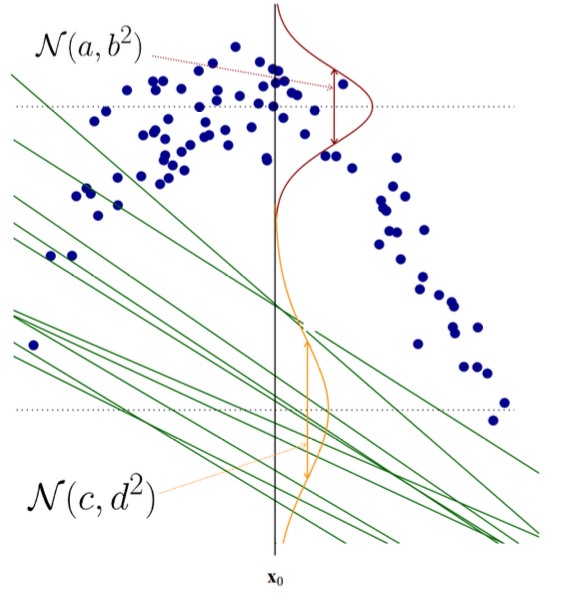
\includegraphics[width=0.7\textwidth]{img/bias-variance.png}
\end{center}

We also use the usual notation convention from the lecture, i.e.:

Let \(Z_l\) be a sample set of \(l\) elements and \(g(x_0; \mathbf{w}(Z_l))\) denote a trained model evaluated at \(x_0\), where the model parameters \(\mathbf{w}\) are dependent on the respective training set \(Z_l\).

Set the variables in the plot as follows:
\[
a = 2, \quad b = 3, \quad c = 1, \quad d = 4
\]

Compute the values of the following terms:
\begin{enumerate}
    \item What is the model variance at \(x_0\)?
    \item What is the unavoidable error at \(x_0\)?
    \item What is \(\mathbb{E}_{y|x_0}(y) - \mathbb{E}_{Z_l}(g(x_0; \mathbf{w}(Z_l)))\)?
    \item What is the expected prediction error at \(x_0\)?
\end{enumerate}

\textit{Provide your answers as integers where applicable or real numbers rounded to two decimal places.}


\subsection*{Binary Classification and Convex Hulls in \(\mathbb{R}^2\)}

Consider the following binary classification problem in \(\mathbb{R}^2\):

The points \((x_1, x_2)\) labeled with \(+1\) are:
\[
\{(2, 2), (1, 2), (1, 1), (2, 1)\}
\]

The points \((x_1, x_2)\) labeled with \(-1\) are:
\[
\{(5, 4), (8, 4), (8, 9), (6, 6)\}
\]

\textbf{Note:} Provide your answers as real numbers rounded to two decimal places. Use ``.'' for the decimal point. Number format example: 0.67.

\begin{enumerate}
    \item What is the area of the convex hull of the points labeled with \(-1\)?
    \item What is the area of the convex hull of the points labeled with \(+1\)?
    \item Compute the separating line given by the linear SVM solution in the form \(x_2 = k \cdot x_1 + d\):
    \begin{enumerate}
        \item Value of \(k\)
        \item Value of \(d\)
    \end{enumerate}
\end{enumerate}



\end{document}
